\documentclass{article}

\usepackage{amsfonts}
\usepackage{pdfpages}
\usepackage[margin=1in]{geometry}

\title{ STAT 321: Assignment 2}
\author{Saksham Sudershan}
\date{07 February 2022}

\begin{document}
	\maketitle

	\section*{Problem 1}
		\subsection*{(a)}
			We know that $P(A)=0.01$, $P(B)=0.005$ and $P(C)=0.02$.
			Let S by the event that a person shows symptoms. And we also know $P(S|A)=1-0.1=0.9$, $P(S|B)=1-0.05 = 0.95$ and $P(S|C)=1-0.25=0.75$.
			Let E' respresent the complement of event E.


			$$ P(S) = P(S|A) \cdot P(A) + P(S|B) \cdot P(B) +  P(S|C) \cdot P(C) $$
			$$ P(S) = 0.9 \cdot 0.01 + 0.95 \cdot 0.005 + 0.75 \cdot 0.02 $$
			$$ P(S) = 0.009+0.00475+0.015$$
			$$ P(S) = 0.02875 $$


			Using Bayes Theorem,
			$$ P(A|S) = \frac{P(S|A) \cdot P(A)}{P(S)}= \frac{0.009}{0.02875}$$
			$$ P(A|S) = 0.313$$

			
			$$ P(B|S) = \frac{P(S|B) \cdot P(B)}{P(S)}= \frac{0.00475}{0.02875}$$
			$$ P(B|S) = 0.165$$


			$$ P(C|S) = \frac{P(S|C) \cdot P(C)}{P(S)}= \frac{0.015}{0.02875}$$
			$$ P(C|S) = 0.522$$

		\subsection*{(b)}
			$$ P(S') = 1-0.02875=0.97125 $$
			
			$$ P(A|S') = \frac{P(S'|A) \cdot P(A)}{P(S')}= \frac{0.1 \cdot 0.01}{0.97125}$$
			$$ P(A|S') = 0.00103 $$


			$$ P(B|S') = \frac{P(S'|B) \cdot P(B)}{P(S')}= \frac{0.05 \cdot 0.005}{0.97125}$$
			$$ P(B|S') = 0.00026 $$


			$$ P(C|S') = \frac{P(S'|C) \cdot P(C)}{P(S')}= \frac{0.25 \cdot 0.02}{0.97125}$$
			$$ P(C|S') = 0.00515 $$

		\subsection*{(c)}
			$$ Sensitivity\ : \; P(T_{+}|A) = 0.95 $$
			$$Specificity\ : \; P(T_{-}|A') = 0.90 $$

			(i)

			$$ P(A'|T_{-}) = \frac{P(T_{-}|A') \cdot P(A')}{P(T_{-})} $$
			$$ P(T_-) = P(T_-|A) \cdot P(A)+P(T_-|A')P(A') = 0.05 \times 0.01 + 0.90 \times 0.99  = .8915 $$
			$$ So\ P(A'|T_{-}) = \frac{0.90 \cdot 0.99}{0.8915}$$
			$$ P(A'|T_{-}) = 0.99944 $$

			(ii)

			For probability of a screening error based on the given test,
			$$ P(Error) = P(T_-|A) \cdot P(A) + P(T_+|A') \cdot P(A') $$
			$$ P(Error) = 0.05 \cdot 0.01 + 0.10 \cdot 0.99 $$
			$$ P(Error) = 0.0995 $$

	\section*{Problem 2}
		\subsection*{(a)}
			Let $R_i$ represent picking a red ball on the $i^{th}$ draw and $B_i$ represent picking a blue ball on the $i^{th}$ draw. Then using the multiplicative rule,
			
			$$ P(X_3 = 4) = P( B_1 \cap B_2 \cap B_3) $$
			$$P(X_3 = 4) = P( B_3|B_1 \cap B_2)\cdot P(B_2|B_1 )\cdot P(B_1) $$ 
			$$P(X_3 = 4) = \frac{5}{8}\cdot \frac{3}{5}\cdot \frac{1}{2} = 0.1875 $$

			$$ P(X_3 = 5) = P[(R_1 \cap B_2 \cap B_3) \cup (B_1 \cap R_2 \cap B_3) \cup (B_1 \cap B_2 \cap R_3)] $$
			$$ P(X_3 = 5) =  P( B_3|R_1 \cap B_2)\cdot P(B_2|R_1 )\cdot P(R_1) +  P( B_3|B_1 \cap R_2)\cdot P(R_2|B_1 )\cdot P(B_1) + P(R_3|B_1 \cap B_2)\cdot P(B_2|B_1 )\cdot \									(B_1) $$ 
			$$P(X_3 = 5) = \frac{4}{8}\cdot \frac{2}{5}\cdot \frac{1}{2} + \frac{4}{8}\cdot \frac{2}{5}\cdot \frac{1}{2} +\frac{3}{8}\cdot \frac{3}{5}\cdot \frac{1}{2}  $$
			$$P(X_3 = 5) = 0.3125 $$

			$$ P(X_3 = 6) = P[(R_1 \cap R_2 \cap B_3) \cup (R_1 \cap B_2 \cap R_3) \cup (B_1 \cap R_2 \cap R_3)] $$
			$$ P(X_3 = 6) =  P( B_3|R_1 \cap R_2)\cdot P(R_2|R_1 )\cdot P(R_1) +  P( R_3|R_1 \cap B_2)\cdot P(B_2|R_1 )\cdot P(R_1) + P(R_3|B_1 \cap R_2)\cdot P(R_2|B_1 )\cdot \									(B_1) $$ 
			$$P(X_3 = 6) = \frac{3}{8}\cdot \frac{3}{5}\cdot \frac{1}{2} + \frac{4}{8}\cdot \frac{2}{5}\cdot \frac{1}{2} +\frac{4}{8}\cdot \frac{2}{5}\cdot \frac{1}{2}  $$
			$$P(X_3 = 6) = 0.3125 $$

			$$ P(X_3 =7) = P(R_1 \cap R_2 \cap R_3) $$
			$$P(X_3 = 7) = P( R_3|R_1 \cap R_2)\cdot P(R_2|R_1 )\cdot P(R_1) $$
			$$P(X_3 = 7) = \frac{5}{8}\cdot \frac{3}{5}\cdot \frac{1}{2} = 0.1875 $$

			So we have,
			$$ P(X_3 = 4)= 0.1875 $$
			$$ P(X_3 = 5)= 0.3125$$
			$$ P(X_3 = 6)= 0.3125$$
			$$ P(X_3 = 7)= 0.1875$$

		\subsection*{(b)}
			$$ \emph{E}(X_3) = \sum_{i=4}^7 P(X_3=i) $$
			$$ \emph{E}(X_3) = 4 \times 0.1875 + 5 \times 0.3125 + 6 \times 0.3125 + 7 \times 0.1875 $$
			$$ \emph{E}(X_3) = 5.5 $$

			$$ Var[X_3] = \emph{E}(X_3^2) - \emph{E}(X_3)^2 $$
			$$ Var[X_3] = 31.25 - 30.25 $$
			$$ Var[X_3] = 1 $$

		\subsection*{(c)}
			For Conditional Probabilities,

			$$ P(R_1|X_3 = 5) = \frac{P(R_1 \cap B_2 \cap B_3)}{P(X_3 = 5)}$$
			$$ P(R_1|X_3 = 5) = \frac{\frac{4}{8}\cdot \frac{2}{5}\cdot \frac{1}{2}}{0.3125}$$
			$$ P(R_1|X_3 = 5) = \frac{0.1}{0.31250}  = 0.32 $$


	\section*{Problem 3}
		\subsection*{(a)}
			Let $S_T$ be the value of stock $S$ after $T$ days. Then,
			$$ P(S_5=23|S_{10}=26) = \frac{P(S_5 = 23 \cap S_{10}=26)}{P(S_{10}=26)} $$
			$$ P(S_5=23|S_{10}=26) = \frac{{5 \choose 4} \cdot p^4 (1-p)^1 \times {5 \choose 4}\cdot p^4 (1-p)^1 }{{10 \choose 8}\cdot p^8 (1-p)^2} $$

		\subsection*{(b)}
			$50p$ is the expected number of stocks that go up in 1 day, and $50 \times (1-p)$ is the expected number of stocks that decrease in value in 1 day.
			
			$$ Expected\ Gain/Loss\ in\ 1\ Day = 50p \cdot 1 \$ + 50(1-p) \cdot -1 \$ $$ 
			$$Expected\ Gain/Loss\ in\ 1\ Day = 50p - 50 +50p = 100p-50 $$

			Now over T days,
	
			$$Expected\ Gain/Loss\ in\ T\ Days = T \times (100p -50) $$
			$$ Expected\ Value\ of\ Portfolio\ in\ T\ Days = 1000+ 100pT - 50T $$

			Since only $p$ is a random variable,
			$$ Var[Portfolio] = 100^2\cdot Var[p]$$
			$$ Var[Portfolio] = 100^2\cdot [p\cdot 1-p]$$
			$$ SD[Portfolio] = 100 \sqrt{p - p^2}$$
		\subsection*{(c)}
			In finance, it is usually important to decrease the risk by minimizing variance by choosing stocks with negative correlations. However, in this scenario, the stocks are all 					independent and so it makes no difference whether 50 stocks of the same company are chosen or if stocks of 50 different companies are chosen. The expected value and SD 				will still be given by,
			$$ \emph{E}[Portfolio] = 1000+ 100pT - 50T $$ 
			$$ SD[Portfolio] = 100 \sqrt{p - p^2}$$
	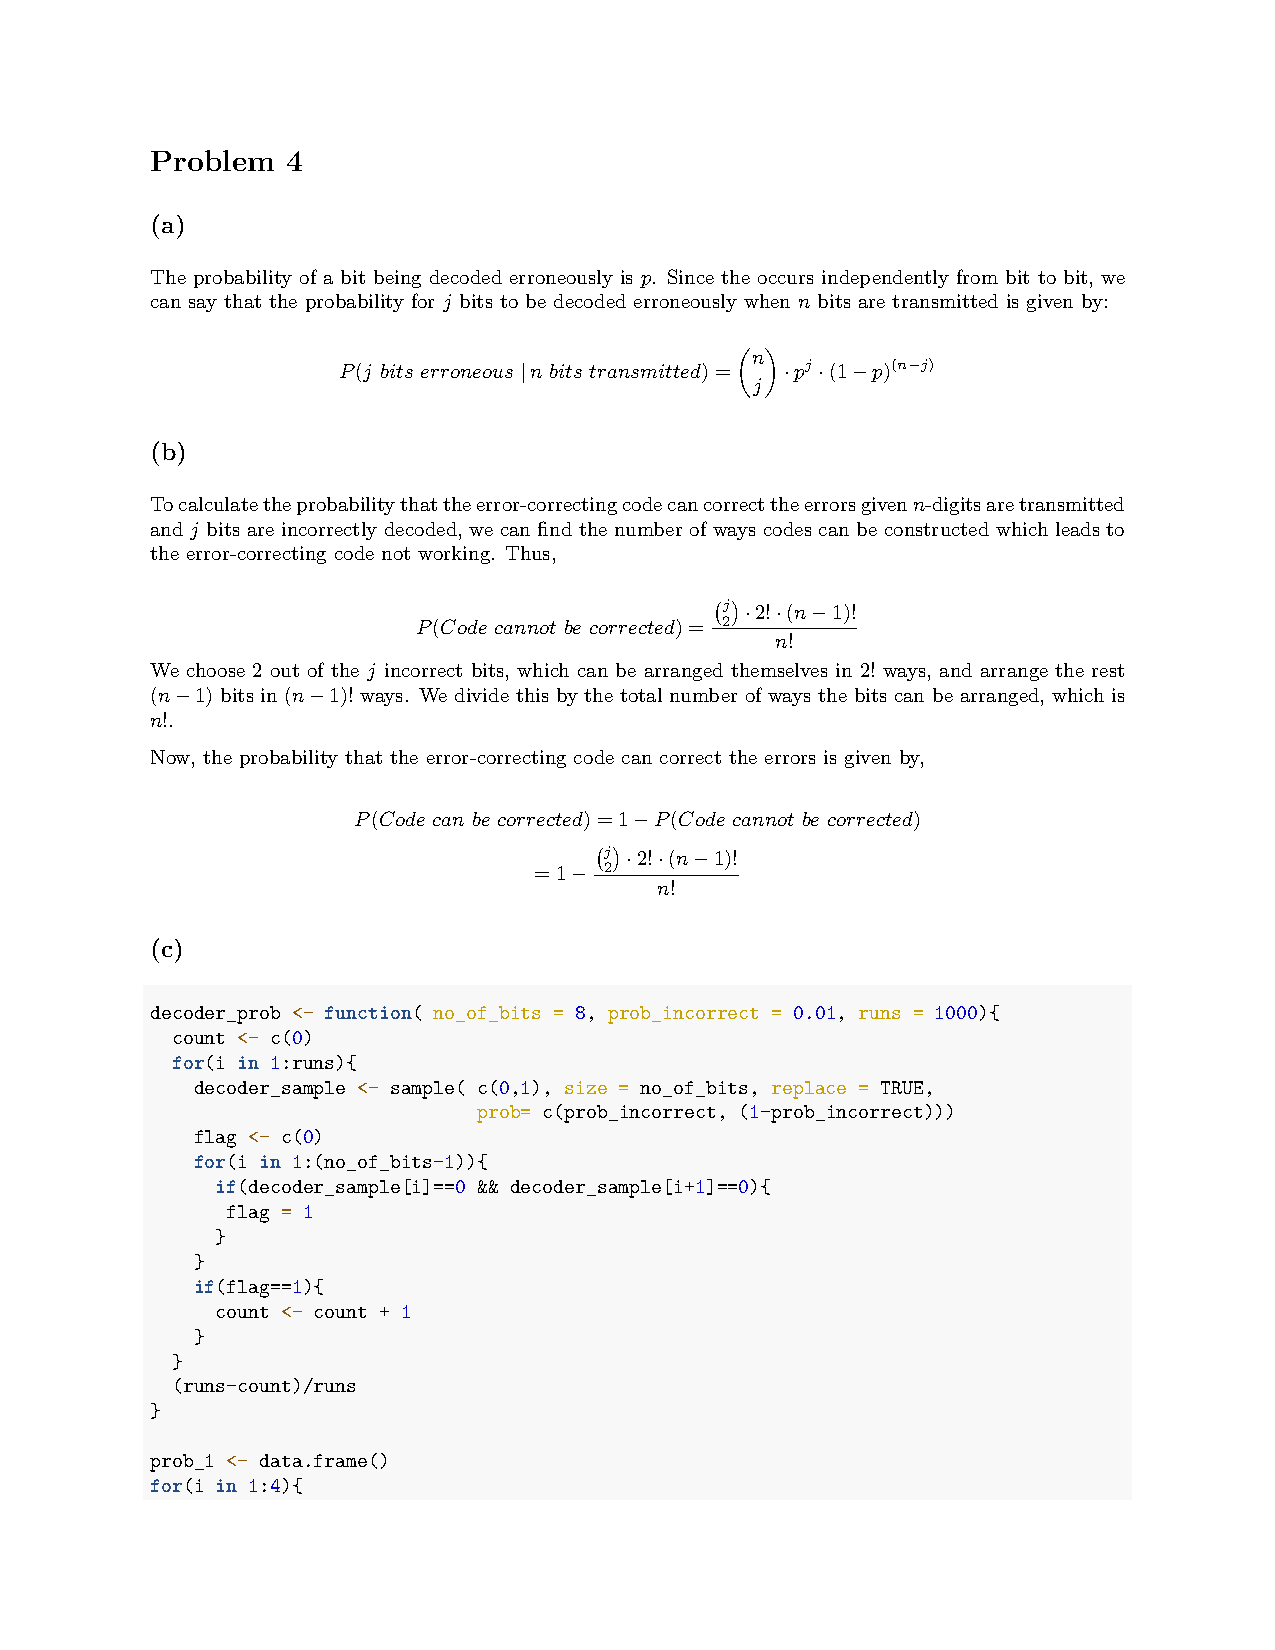
\includepdf[pages=-, pagecommand={}]{Assign-2-Part-2.pdf}
\end{document}